% ====================================================
%  组会汇报 Beamer 模板
%  Author: 葛良晨
%  Compile: latexmk -xelatex -shell-escape
% ====================================================
\documentclass[aspectratio=169, 10pt, UTF8]{ctexbeamer}

% ---------- 主题 ----------
\usetheme{Madrid}
\usecolortheme{default}

% ---------- 颜色定义 ----------
\definecolor{ieeeBlue}{RGB}{0, 83, 159}
\definecolor{ieeeRed}{RGB}{198, 38, 46}
\definecolor{ieeeGreen}{RGB}{0, 114, 41}
\definecolor{ieeeOrange}{RGB}{235, 110, 31}
\definecolor{darkGray}{RGB}{66, 66, 66}

\setbeamercolor{structure}{fg=ieeeBlue}
\setbeamercolor{alerted text}{fg=ieeeRed}
\setbeamercolor{example text}{fg=ieeeGreen}
\setbeamercolor{frametitle}{bg=ieeeBlue!15, fg=ieeeBlue}
\setbeamercolor{block title}{bg=ieeeBlue!15, fg=ieeeBlue}
\setbeamercolor{block body}{bg=ieeeBlue!5}
\setbeamercolor{block title example}{bg=ieeeGreen!15, fg=ieeeGreen}
\setbeamercolor{block body example}{bg=ieeeGreen!5}
\setbeamercolor{block title alerted}{bg=ieeeRed!15, fg=ieeeRed}
\setbeamercolor{block body alerted}{bg=ieeeRed!5}

% ---------- 包 ----------
\usepackage{graphicx}
\usepackage{booktabs}
\usepackage{tabularx}
\usepackage{listings}
\usepackage{amsmath,amssymb}
% enumitem 与 Beamer 冲突，使用 Beamer 自带的列表系统
\usepackage{tikz}
\usetikzlibrary{positioning, calc, shapes.geometric, arrows.meta, backgrounds, fit, shadows}
\usepackage{pgfplots}
\pgfplotsset{compat=1.18}
\usepackage{hyperref}

% ---------- 代码样式 ----------
\lstset{
  basicstyle=\ttfamily\small,
  frame=single,
  breaklines=true,
  keywordstyle=\color{ieeeBlue},
  commentstyle=\color{ieeeGreen},
  stringstyle=\color{ieeeRed},
  numbers=left,
  numberstyle=\tiny\color{gray},
  numbersep=5pt,
  backgroundcolor=\color{gray!5}
}

% ---------- 元信息 ----------
\title[组会汇报模板]{组会学术汇报模板 \\[4pt] {\normalsize\color{darkGray} —— 功能演示与快速上手指南}}
\subtitle{Latex Beamer Full Features Demo}
\author[葛良晨]{葛良晨}
\institute[GLC Lab]{某某大学 · 某实验室}
\date{\today}

% ---------- 页脚自定义 ----------
% 显示页码和总页数
\setbeamertemplate{footline}[frame number]

\begin{document}

% ============================================
%  Title Slide
% ============================================
\begin{frame}
  \titlepage
\end{frame}

% ============================================
%  目录
% ============================================
\begin{frame}{目录 (Outline)}
  \tableofcontents
\end{frame}

% ================================================================
\section{基础排版元素}
% ================================================================

% ---------- 文本块 ----------
\begin{frame}{块环境 (Block Environments)}
  \begin{block}{普通块 (Block)}
    这是一个普通的信息块，适用于陈述一般性结论。
  \end{block}

  \begin{alertblock}{警告块 (Alert Block)}
    需要注意的关键问题或限制条件。
  \end{alertblock}

  \begin{exampleblock}{示例块 (Example Block)}
    \begin{itemize}
      \item 具体示例、案例或实验结果
      \item 支持列表嵌套
    \end{itemize}
  \end{exampleblock}
\end{frame}

% ---------- 定理环境 ----------
\begin{frame}{定理与定义环境}
  \begin{definition}[信息熵]
    对于离散随机变量 $X$，其信息熵定义为：
    \[
      H(X) = -\sum_{x \in \mathcal{X}} p(x) \log_2 p(x)
    \]
  \end{definition}

  \begin{theorem}[No-Free-Lunch Theorem]
    在所有可能的优化问题上，没有任何算法平均表现优于其他算法。
  \end{theorem}

  \begin{proof}
    基于归纳假设，对所有可能的目标函数取期望即可得证。
  \end{proof}
\end{frame}

% ---------- 列表 ----------
\begin{frame}{列表 (Lists)}
  \begin{columns}[T]
    \begin{column}{0.45\textwidth}
      无序列表：
      \begin{itemize}
        \item 第一层
        \begin{itemize}
          \item 第二层
        \end{itemize}
        \item 另一个要点
      \end{itemize}
    \end{column}

    \begin{column}{0.45\textwidth}
      有序列表：
      \begin{enumerate}
        \item 准备工作
        \item 核心方法
        \begin{enumerate}
          \item 子步骤 A
          \item 子步骤 B
        \end{enumerate}
        \item 结果分析
      \end{enumerate}
    \end{column}
  \end{columns}

  \vspace{12pt}
  \begin{alertblock}{Tip}
    用 \texttt{columns} 环境实现并排列表，节省纵向空间。
  \end{alertblock}
\end{frame}

% ---------- 公式 ----------
\begin{frame}{数学公式}
  行内公式：$\sigma(x) = \frac{1}{1 + e^{-x}}$ 可以嵌入正文。

  行间公式（带编号）：
  \begin{equation}
    \mathcal{L}(\theta) = -\frac{1}{N} \sum_{i=1}^{N} \log P(y_i \mid x_i; \theta) \label{eq:loss}
  \end{equation}

  多行公式：
  \begin{align}
    \text{Attention}(Q, K, V) &= \text{softmax}\!\left(\frac{QK^\top}{\sqrt{d_k}}\right) V \\
    \text{MultiHead}(Q, K, V) &= \text{Concat}(\text{head}_1, \ldots, \text{head}_h) W^O
  \end{align}

  \begin{exampleblock}{交叉引用}
    公式~\eqref{eq:loss} 是标准的交叉熵损失函数。
  \end{exampleblock}
\end{frame}

% ================================================================
\section{表格与数据}
% ================================================================

\begin{frame}{表格 (Tables)}
  \begin{table}[h]
    \centering
    \caption{各方法在 Benchmark 上的性能对比}
    \begin{tabular}{l c c c}
      \toprule
      方法 & 准确率 (\%) & 参数量 (M) & 推理时延 (ms) \\
      \midrule
      ResNet-50  & 76.15 & 25.6 & 12.3 \\
      ViT-B/16   & 78.82 & 86.4 & 18.7 \\
      \textbf{Our Method} & \textbf{80.34} & 42.1 & 14.1 \\
      \bottomrule
    \end{tabular}
  \end{table}

  \begin{itemize}
    \item 用 \texttt{\textbackslash{}textbf} 加粗最优结果
    \item \texttt{booktabs} 三线表风格，避免竖线
  \end{itemize}
\end{frame}

% ================================================================
\section{图形}
% ================================================================

% ---------- TikZ 流程图 ----------
\begin{frame}{TikZ 流程图}
  \begin{figure}[h]
    \centering
    \begin{tikzpicture}[
      node distance=8mm and 15mm,
      block/.style={rectangle, draw=ieeeBlue, rounded corners=3pt, minimum width=20mm, minimum height=8mm, fill=ieeeBlue!10},
      arrow/.style={-{Stealth[scale=1.2]}, thick, ieeeBlue}
    ]
      % 使用相对定位，禁止魔数坐标
      \node[block] (input) {输入数据};
      \node[block, right=of input] (enc) {特征编码};
      \node[block, right=of enc] (core) {核心模块};
      \node[block, below=of core] (aux) {辅助分支};
      \node[block, right=of core] (dec) {解码输出};
      \node[block, right=of dec] (out) {结果};

      \draw[arrow] (input) -- (enc);
      \draw[arrow] (enc) -- (core);
      \draw[arrow] (core) -- (aux);
      \draw[arrow] (aux) -- (dec);
      \draw[arrow] (core) -- (dec);
      \draw[arrow] (dec) -- (out);
    \end{tikzpicture}
    \caption{系统流程图 (TikZ 相对定位)}
  \end{figure}
\end{frame}

% ---------- pgfplots 数据图 ----------
\begin{frame}{PGFPlots 数据绘图}
  \begin{figure}[h]
    \centering
    \begin{tikzpicture}
      \begin{axis}[
        width=0.8\textwidth,
        height=0.55\textheight,
        xlabel={训练轮次 (Epoch)},
        ylabel={准确率 (\%)},
        grid=major,
        legend pos=south east,
        cycle list={{ieeeBlue},{ieeeRed},{ieeeGreen}}
      ]
      \addplot coordinates {(1,60)(2,72)(3,78)(4,82)(5,85)(6,87)(7,88)};
      \addlegendentry{Our Method}

      \addplot coordinates {(1,55)(2,65)(3,70)(4,74)(5,77)(6,79)(7,80)};
      \addlegendentry{Baseline A}

      \addplot coordinates {(1,50)(2,58)(3,63)(4,67)(5,70)(6,72)(7,73)};
      \addlegendentry{Baseline B}
      \end{axis}
    \end{tikzpicture}
    \caption{训练曲线对比 (pgfplots)}
  \end{figure}
\end{frame}

% ---------- 子图 ----------
\begin{frame}{并排子图 (Subfigures)}
  \begin{figure}[h]
    \centering
    \begin{minipage}{0.48\textwidth}
      \centering
      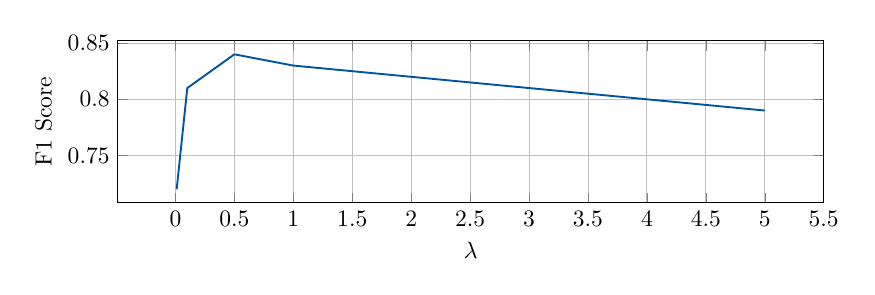
\begin{tikzpicture}[scale=0.85]
        \begin{axis}[
          width=\textwidth,
          height=40mm,
          xlabel={$\lambda$},
          ylabel={F1 Score},
          grid=major
        ]
        \addplot[ieeeBlue, thick] coordinates {(0.01,0.72)(0.1,0.81)(0.5,0.84)(1.0,0.83)(5.0,0.79)};
        \end{axis}
      \end{tikzpicture}
      \subcaption{超参数 $\lambda$ 的影响}
    \end{minipage}
    \hfill
    \begin{minipage}{0.48\textwidth}
      \centering
      \begin{tikzpicture}[scale=0.85]
        \begin{axis}[
          width=\textwidth,
          height=40mm,
          xlabel={Batch Size},
          ylabel={吞吐量 (samples/s)},
          grid=major
        ]
        \addplot[ieeeRed, thick] coordinates {(8,120)(16,210)(32,350)(64,480)};
        \end{axis}
      \end{tikzpicture}
      \subcaption{Batch Size 对吞吐量的影响}
    \end{minipage}
    \caption{消融实验结果}
  \end{figure}
\end{frame}

% ================================================================
\section{代码展示}
% ================================================================

\begin{frame}[fragile]{代码块展示 (Code Listings)}
  \begin{lstlisting}[language=Python, caption={PyTorch 训练循环示例}]
def train_one_epoch(model, loader, optimizer):
    model.train()
    total_loss = 0
    for x, y in loader:
        optimizer.zero_grad()
        logits = model(x)
        loss = F.cross_entropy(logits, y)
        loss.backward()
        optimizer.step()
        total_loss += loss.item()
    return total_loss / len(loader)
  \end{lstlisting}

  \begin{alertblock}{注意}
    使用 \texttt{fragile} 帧选项以确保 \texttt{lstlisting}/\texttt{verbatim} 正确渲染。
  \end{alertblock}
\end{frame}

% ================================================================
\section{参考文献}
% ================================================================

\begin{frame}[allowframebreaks]{参考文献 (References)}
  \begin{thebibliography}{10}
    \beamertemplatebookbibitems

    \bibitem{vaswani2017}
    A.~Vaswani et al.
    \newblock {\em Attention Is All You Need}.
    \newblock NeurIPS, 2017.

    \bibitem{he2016}
    K.~He et al.
    \newblock {\em Deep Residual Learning for Image Recognition}.
    \newblock CVPR, 2016.

    \bibitem{devlin2019}
    J.~Devlin et al.
    \newblock {\em BERT: Pre-training of Deep Bidirectional Transformers}.
    \newblock NAACL, 2019.

    \bibitem{brown2020}
    T.~Brown et al.
    \newblock {\em Language Models are Few-Shot Learners}.
    \newblock NeurIPS, 2020.
  \end{thebibliography}
\end{frame}

% ================================================================
%  结束页
% ================================================================
\begin{frame}[plain]
  \centering
  \vfill
  {\huge\color{ieeeBlue} 谢谢！欢迎提问}

  \vspace{20pt}
  {\large 邮箱：example@university.edu.cn}

  \vspace{8pt}
  {\large GitHub：\href{https://github.com/username}{github.com/username}}
  \vfill
\end{frame}

\end{document}
